\chapter{Fundamentação Teórica}

Este capítulo estabelece o embasamento teórico necessário para o desenvolvimento do projeto. Inicialmente, abordam-se os princípios da robótica móvel aplicada à educação e a caracterização da plataforma robótica utilizada. Em seguida, são apresentados os fundamentos da modelagem cinemática para robôs com tração diferencial, o protocolo de comunicação Bluetooth Low Energy (BLE) e, por fim, o desenvolvimento de interfaces móveis com o framework Flutter.

\section{Robótica Aplicada à Educação}

O ritmo acelerado da sociedade atualmente não permite que a educação


\section{Características e Aplicação Educacional do Robô Juca}

O robô Juca é uma plataforma robótica móvel embarcada desenvolvida no Instituto Federal de Santa Catarina (IFSC) com o objetivo principal de servir como ferramenta de ensino e aprendizado prático (hands-on learning) em engenharia, sistemas embarcados e robótica móvel


 \begin{citacao}
            \begin{alineas}[leftmargin=\leftskip+\labelwidth-\labelsep]
                Texto texto texto texto texto texto texto texto. Texto texto texto texto texto texto. Texto texto texto texto texto texto texto texto texto. Texto texto texto texto texto texto Texto texto texto texto texto texto. Texto texto texto texto texto texto. (\citeauthor{ref:ibmm}, \citeyear{ref:ibmm}, p. 20).
            \end{alineas}
\end{citacao}

\section{Robôs móveis com tração diferencial 2WD}

\subsection{Subtítulo Terciário}

Texto texto texto texto texto texto texto texto texto texto texto texto texto texto texto texto texto texto texto texto texto texto texto texto texto texto texto texto texto texto texto texto texto. \cite{ref:mulligan}.

\section{Cinemática Direta e Inversa}

\subsubsection{Subtítulo Quaternário}

Texto texto texto texto texto texto texto texto texto texto texto texto texto texto texto texto texto texto texto texto texto texto texto texto texto texto texto texto texto texto texto texto texto  (conforme exposto na Figura \ref{fig:motor}).



    \begin{figure}[H]
    	\centering
    	\caption{Motor Weg W22}
    	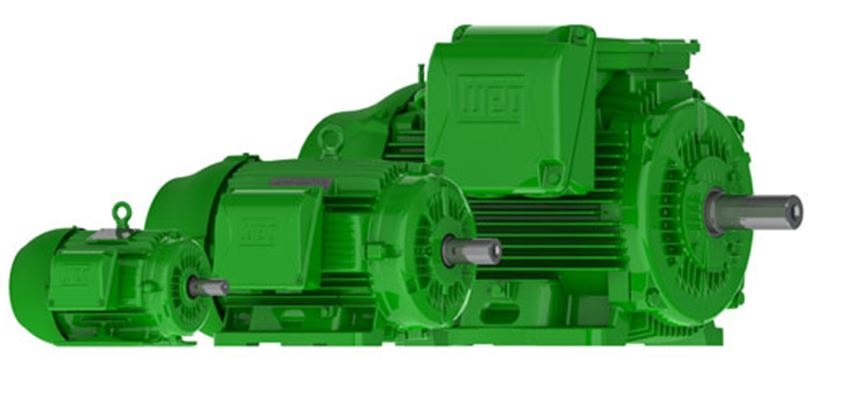
\includegraphics[scale=0.45]{figuras/motor.jpg}
    	\label{fig:motor}
    	\\
        \vspace{-0.8cm}\hspace{-7cm}\small{Fonte: WEG (2014).} 
    \end{figure}
    
    Texto texto texto texto texto texto texto texto texto texto texto texto texto texto texto conforme indica a Tabela \ref{tabela1}.

    

\begin{table}[h]
\centering
\caption{Produção de petróleo na Bahia}
\begin{tabular}{ c c }
\ChangeRT{2pt}
Ano  & Produção (1000 t) \\ \ChangeRT{2pt}
1996 & 2.536             \\ 
1997 & 2.665             \\ 
1998 & 3.056             \\ 
1999 & 3.567             \\ 
2021 & Atômica           \\ \ChangeRT{2pt}
\end{tabular}
\label{tabela1}
\\
\small{Fonte: Adaptado de ANP (2000).} 
\end{table}



    
    Texto texto texto texto texto texto texto texto texto texto texto texto texto texto texto texto texto texto texto texto texto texto texto texto texto texto texto texto texto texto texto texto texto 
    Texto texto texto texto texto texto texto texto texto texto texto texto texto texto texto texto texto texto texto texto texto texto texto texto texto texto texto texto texto texto texto texto texto como evidencia a Figura  \ref{fig:diagrama}.
    
    
    
    \begin{figure}[H]
    	\centering
    	\caption{Diagrama Fasorial}
    	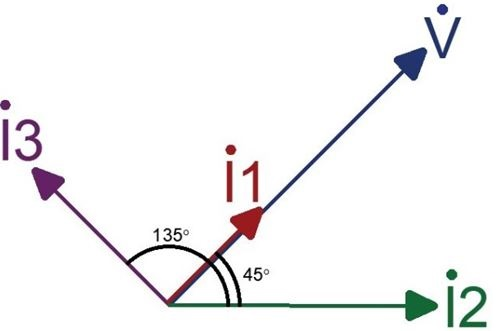
\includegraphics[scale=0.45]{figuras/diagrama.jpg}
    	\label{fig:diagrama}
    	\\
    	\vspace{0.2cm}\hspace{-3cm}\small{Fonte: Silva (2020).}
    \end{figure}
    
    Texto texto texto texto texto texto texto texto texto texto texto texto texto texto texto texto texto texto texto texto texto texto texto texto texto texto texto texto texto texto texto texto, conforme mostra a Equação \ref{eq:baskara}.
    
\begin{equation} \label{eq:baskara}
  x=\frac{-b\pm\sqrt{b^2-4ac}}{2a}
\end{equation} 
